\documentclass[a4paper,twoside,12pt]{article}
\usepackage[top=1.5cm,left=1.5cm,right=1.5cm,bottom=2cm]{geometry}

\usepackage[utf8]{inputenc}
\usepackage[T1]{fontenc}
\usepackage{lmodern}
\usepackage[brazilian]{babel}

\usepackage{graphicx}
\usepackage{subfig}
\usepackage{psfrag}
\usepackage{cite}
\usepackage[cmex10]{amsmath}
\usepackage{amssymb}
\usepackage{upgreek}
\usepackage{microtype}
\usepackage{titling}
\usepackage{courier}
\usepackage{url}
\usepackage{hyperref}
\hypersetup{
	colorlinks=true,
	linkcolor=blue,
	urlcolor=blue
}

% Use o pacote 'listings' para adicionar código e o pacote 'color' para gerar os destaques
\usepackage{listings}
\usepackage{color}
\definecolor{grey}{rgb}{0.6,0.6,0.6}
\definecolor{codegreen}{rgb}{0,0.6,0}
\definecolor{codegray}{rgb}{0.5,0.5,0.5}
\definecolor{codepurple}{rgb}{0.58,0,0.82}
\definecolor{backcolour}{rgb}{0.95,0.95,0.92}
\lstset{language=Python,				% definir para destaque de linguagem Python
	backgroundcolor=\color{backcolour},
	commentstyle=\color{codegreen},
	keywordstyle=\color{magenta},
	numberstyle=\tiny\color{codegray},
	stringstyle=\color{codepurple},
	basicstyle=\ttfamily\small,		% definir tamanho das fontes
	breaklines=true,				% definir quebra de linha automática
	linewidth=\textwidth,			% definir tamanho da caixa de código
	showstringspaces=false}			% mostrar espaços como sublinhados apenas dentro de strings


\title{\vspace{-2cm} Processamento Digital de Sinais\\ Soluções para Tutorial 11 - Periodograma e Método de Welch}
\author{\url{https://github.com/fchirono/Aulas_PDS_Acustica}}

\begin{document}
	\date{}
	\maketitle
	
	
	\setcounter{section}{1}
	\section{Tarefas}
	
	\subsection{Periodograma e Método de Welch}
	
	\subsubsection*{Tarefa 1}
	A Figura \ref{fig:SinaisTempo_T1} compara as primeiras amostras do sinal de ruído branco original com o sinal resultante após a filtragem passa-faixas.
		
	\begin{figure}[h!]
		\centering
		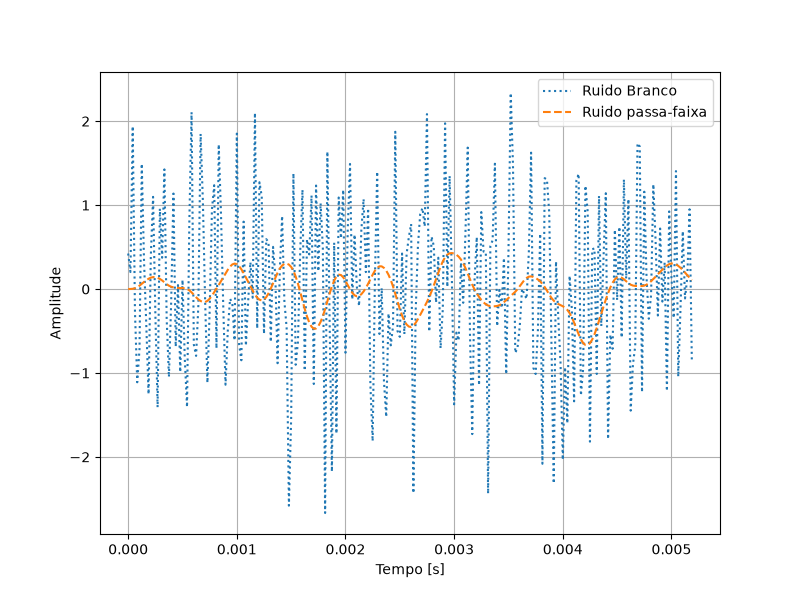
\includegraphics[width = 0.5\textwidth]{SinaisTempo_T1.png}
		\caption{Comparação, no domínio do tempo, entre o sinal de ruído branco original e o sinal filtrado por um passa-faixas Butterworth de 4\textsuperscript{a} ordem ($f_{c,baixa}=50$ Hz, $f_{c,alta}=2000$ Hz).}
		\label{fig:SinaisTempo_T1}
	\end{figure}
	
	\subsubsection*{Tarefa 2}
	-
	
	\subsubsection*{Tarefa 3}
	A Figura \ref{fig:PSD_Periodograma_T2} apresenta a Densidade Espectral de Potência do sinal {\tt x\_passafaixa} estimada pelo periodograma, para diferentes durações $N$ do sinal analisado. Conforme a duração da série temporal analisada aumenta, o estimador tipo periodograma aumenta a resolução em frequência (i.e. diminui a distância entre amostras adjacentes da DFT), mas \textbf{não} reduz a variância da estimativa - as curvas permanecem igualmente ``ruidosas'' (erráticas) independentemente da duração do sinal utilizado. Como consequência, o periodograma não converge para a Densidade Espectral de Potência teórica do sinal conforme mais dados são utilizados.
	
	\begin{figure}[h!]
		\centering
		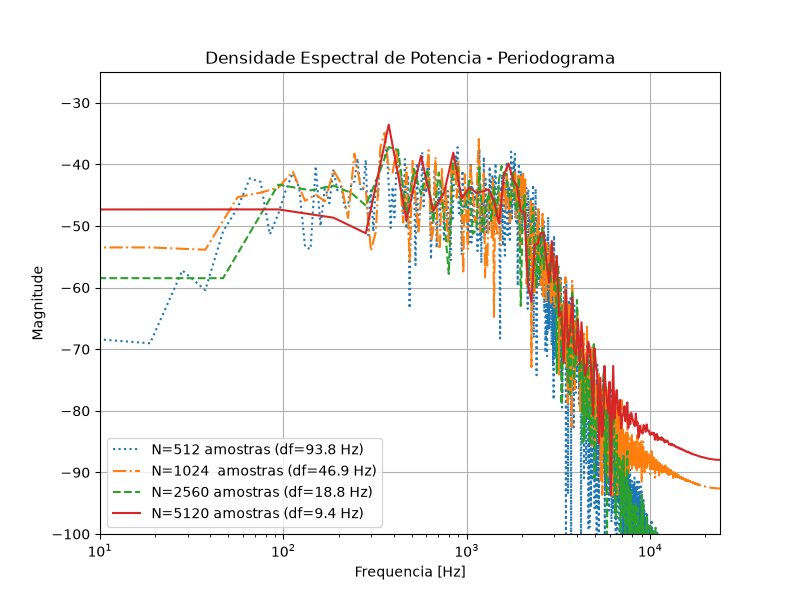
\includegraphics[width = 0.75\textwidth]{PSD_Periodograma_T2.png}
		\caption{Densidade Espectral de Potência do sinal passa-faixa, estimada pelo periodograma, para diferentes durações do sinal (e portanto diferentes resoluções em frequência $\Delta f$).}
		\label{fig:PSD_Periodograma_T2}
	\end{figure}
	
	
	\subsubsection*{Tarefa 4}
	-
	
	\subsubsection*{Tarefa 5}
	A Figura \ref{fig:PSD_Welch_T3} apresenta a Densidade Espectral de Potência do sinal {\tt x\_passafaixa} estimada pelo método de Welch, mantendo $N_{DFT}=512$ e $N_{sobreposicao}=256$ fixos e variando a duração total $N$ do sinal analisado.
	
	\begin{figure}[h!]
		\centering
		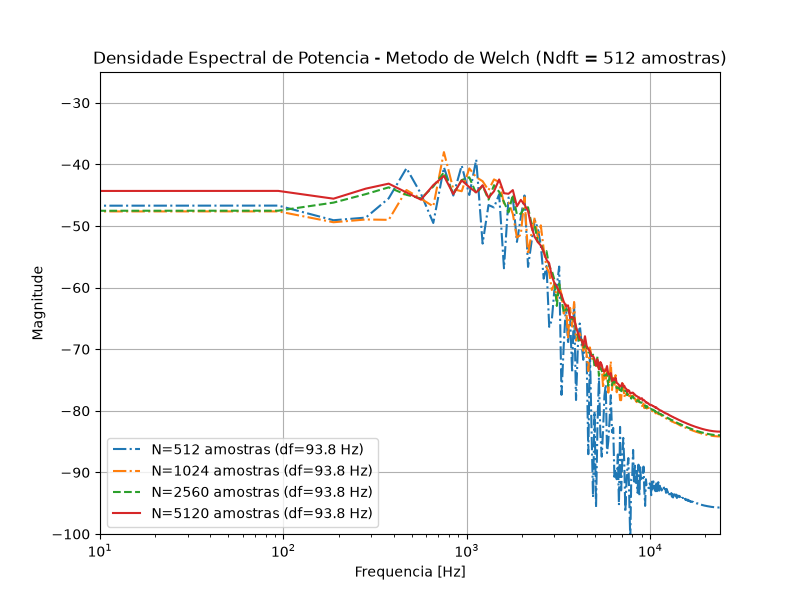
\includegraphics[width = 0.75\textwidth]{PSD_Welch_T3.png}
		\caption{Densidade Espectral de Potência do sinal passa-faixa, estimada pelo método de Welch com $N_{DFT}=512$ fixo, para diferentes durações do sinal analisado (e portanto diferentes números de quadros médios).}
		\label{fig:PSD_Welch_T3}
	\end{figure}
	
	Ao contrário do periodograma, conforme a duração da série temporal aumenta, o estimador de Welch \textbf{não} aumenta a resolução em frequência (que permanece fixa, definida por $N_{DFT}$), mas \textbf{reduz} a variância da estimativa - as curvas ficam visivelmente menos erráticas, dado que séries temporais mais longas resultam em mais quadros utilizados no cálculo do espectro médio. Portanto, o estimador de Welch converge para a Densidade Espectral de Potência teórica do sinal conforme mais dados são utilizados.
	
	\textbf{Nota:} neste caso em particular, o número de pontos da DFT não resulta em uma resolução em frequência (aprox. 94 Hz) fina o bastante para ``resolver'' a frequência de corte inferior (50 Hz) do filtro passa-faixas. Para melhor observar este efeito, seria necessário aumentar o tamanho da DFT.
	
	\newpage
	\clearpage 
	
	\subsection{Espectro de Potência (PS) e Densidade Espectral de Potência (PSD)}
	
	\subsubsection*{Tarefa 1}
	-
	
	\subsubsection*{Tarefa 2}
	A Figura \ref{fig:PSD_Welch_Ndft_T4} apresenta a Densidade Espectral de Potência do sinal {\tt x\_soma} (senoide + ruído passa-faixa), estimada pelo método de Welch com janela de Hann, para diferentes valores de $N_{DFT}$. Note que a duração total do sinal $N$ é mantida constante.
	
	\begin{figure}[h!]
		\centering
		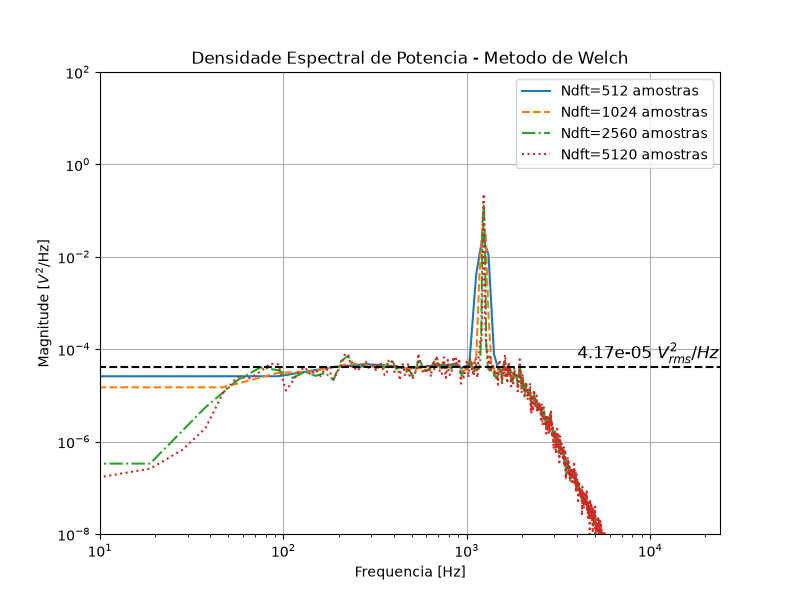
\includegraphics[width = 0.75\textwidth]{PSD_Welch_Ndft_T4.png}
		\caption{Densidade Espectral de Potência do sinal {\tt x\_soma}, estimada pelo método de Welch, para diferentes valores de $N_{DFT}$.}
		\label{fig:PSD_Welch_Ndft_T4}
	\end{figure}
	
	A Densidade Espectral de Potência resulta em uma estimativa correta e consistente da densidade de potência do sinal uído branco ($2 \sigma^2/fs \approx 4.17 \cdot 10^{-5}\  V^2/Hz$) dentro da faixa de passagem, \emph{independentemente} da escolha de $N_{DFT}$. 
	
	Por outro lado, a magnitude do pico correspondente à densidade de potência do sinal senoidal varia com a escolha de $N_{DFT}$. Isso ocorre porque cada elemento da PSD corresponde à potência total contida dentro de uma ``bin'' (``caixinha'') de largura $\Delta f = f_s/N_{DFT}$, dividida pela largura $\Delta f = f_s/N_{DFT}$ da caixinha. Assim, a magnitude do pico da PSD é proporcional à potência do sinal senoidal (que é concentrada em uma única frequência de largura infinitesimal) dividido pela largura $\Delta f$ da ``bin'' contendo o sinal senoidal.
	
	\subsubsection*{Tarefa 3}
	A Figura \ref{fig:PS_Welch_Ndft_T5} apresenta o Espectro de Potência (ao invés da Densidade Espectral de Potência) do mesmo sinal {\tt x\_soma}, para os mesmos valores de $N_{DFT}$ utilizados na Tarefa 7. A linha tracejada horizontal indica o valor teórico $V^2 = 4 \ V^2_{rms}$ da potência do sinal senoidal. Note que a duração total do sinal $N$ é mantida constante.
	
	\begin{figure}[h!]
		\centering
		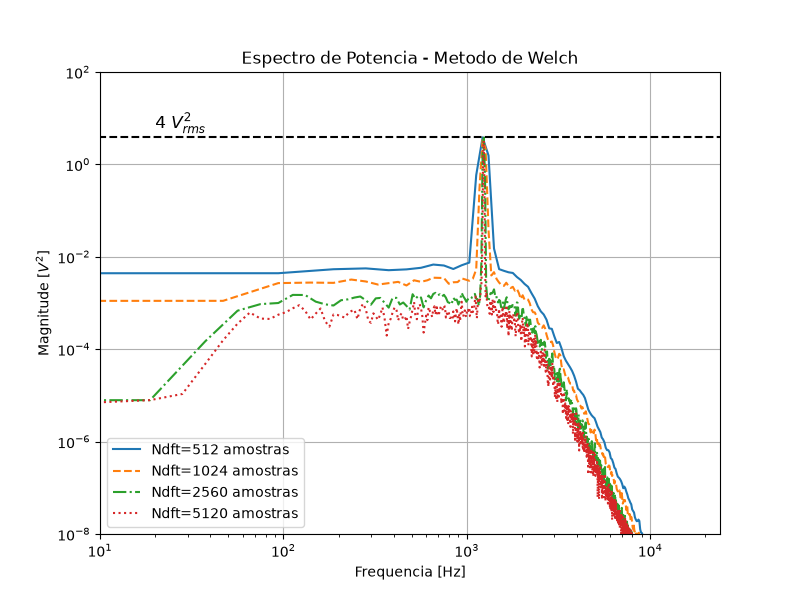
\includegraphics[width = 0.75\textwidth]{PS_Welch_Ndft_T5.png}
		\caption{Espectro de Potência do sinal {\tt x\_soma}, estimado pelo método de Welch, para diferentes valores de $N_{DFT}$. A linha tracejada indica o valor teórico $V_{rms}^2$ do sinal senoidal.}
		\label{fig:PS_Welch_Ndft_T5}
	\end{figure}
	
	O Espectro de Potência resulta em uma estimativa correta e consistente da potência do sinal senoidal ($V_{rms}^2$), \emph{independentemente} da escolha de $N_{DFT}$: o pico coincide com o valor teórico a em todos os quatro casos. Por outro lado, o valor de potência associado ao patamar de ruído passa-faixa varia com $N_{DFT}$: resoluções em frequência mais grosseiras (i.e. $N_{DFT}$ menores, ``bins'' largas) resultam em mais energia por caixinha, enquanto resoluções mais finas (i.e. $N_{DFT}$ maiores, ``bins'' estreitas) resultam em menos energia por caixinha.
	
	\subsubsection*{Tarefa 4}
	A duração total $N$ do sinal analisado é mantida constante em todos os casos; portanto, valores menores de $N_{DFT}$ geram um número maior de quadros (janelas) curtos, resultando em mais elementos disponíveis para o cálculo da média do espectro, e portanto em uma estimativa com menor variância (menos errática) e com resolução em frequência grosseira ($\Delta f$ grande). Por outro lado, valores maiores de $N_{DFT}$ resultam em um número menor de quadros calculados e, portanto, em menos elementos disponíveis para a média, resultando em uma estimativa com maior variância (mais ``errática''/ruidosa)  e com resolução em frequência mais fina ($\Delta f$ pequena).
	
	Este é precisamente o compromisso fundamental do método de Welch: dada uma duração fixa de sinal, é preciso escolher entre melhor resolução em frequência (usando $N_{DFT}$ maior, com menos quadros médios) ou menor variância da estimativa espectral (usando $N_{DFT}$ menor, com mais quadros médios).
	
\end{document}